\subsection{High-level Overview}

\begin{figure*}[]
\caption{DiffTrace Overview}
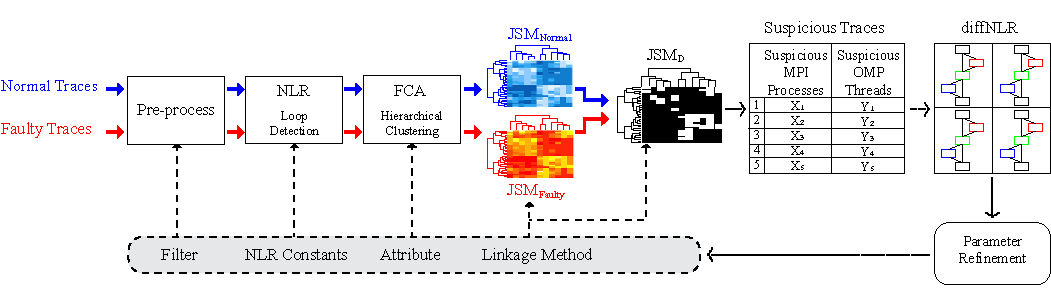
\includegraphics[width=1\textwidth]{figs/overview4.pdf}
%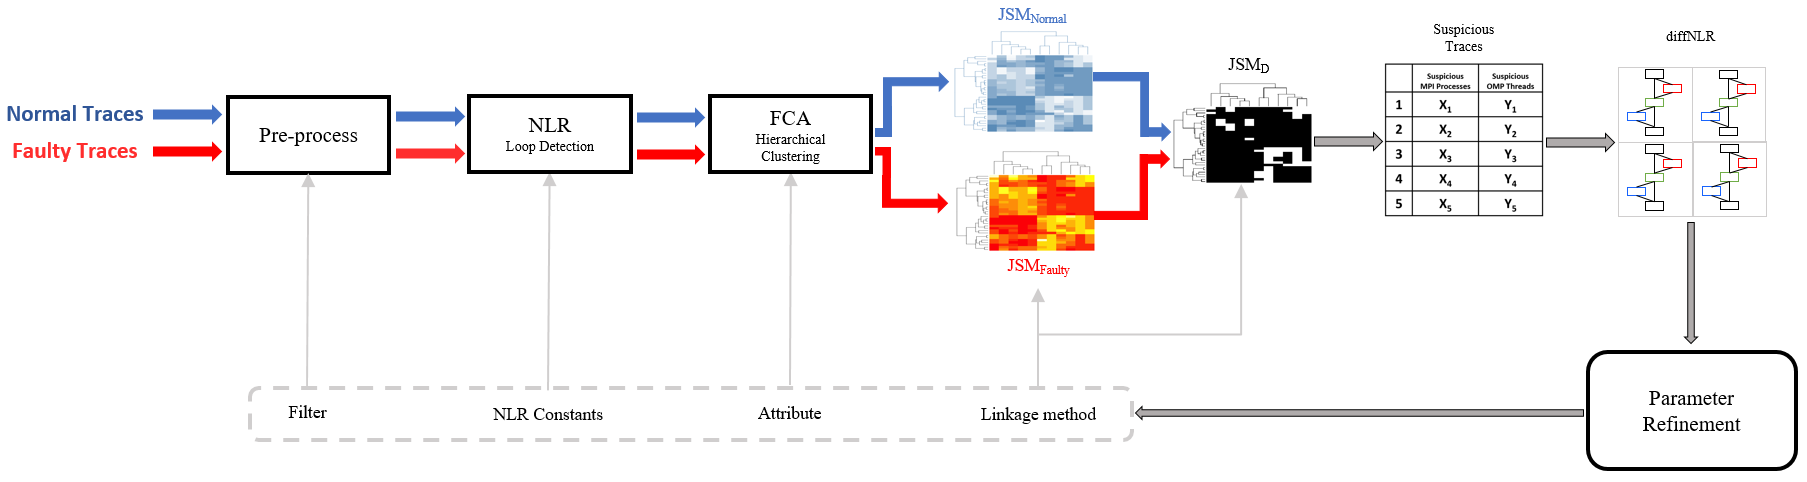
\includegraphics[]{figs/overview.png}
%\includegraphics[]{figs/overv}
\label{fig.diffTraceOverview}
\end{figure*}

DiffTrace employs ParLoT's whole-program function-call and return trace-collection mechanism, where ParLoT captures traces via Pin~\cite{pin} and incrementally compresses them using a new compression scheme~\cite{parlot}.
%
ParLoT can capture functions at two levels:
the \textit{main image} (which does not include library code)
and \textit{all images} (including all application code).
%
As the application runs,
ParLoT generates per-thread trace files that
contain the compressed sequence of the IDs of the executed functions.
%
The compression mechanism is light-weight yet effective,
thus reducing not only the required bandwidth and storage but also the
runtime relative to not compressing the traces.
As a result, ParLoT can capture whole-program traces at low overhead
while leaving most of the disk bandwidth to the application. 
%
Using whole-program traces substantially reduces the number of overall
debug iterations because it allows us to repeatedly analyze the
traces offline with different filters.


Figure \ref{fig.diffTraceOverview} provides an overview
of the DiffTrace toolchain
in terms of the blue flows (fault-free) and red flows
(faulty).
%
In a broad sense,
code-level faults in HPC applications (e.g.,
the use of wrong subscripts) turn into observable code-level
misbehaviors
(e.g., an unexpected number of loop iterations), many of which
turn into application-level issues.
%
In our study of DiffTrace, we evaluate
success merely in terms of the efficacy of observing
these misbehaviors in response to injected code-level
faults (we rely on a rudimentary fault injection framework
complemented by manual fault injection).

The preprocessing stage removes calls/returns at the ignored APIs.
%
The nested loop recognition (NLR)
mechanism then extracts loops from traces.
The resulting information not only
serves as a lossless abstraction to
ease the rest of the trace analysis but also
serves as a {\em per-thread measure of progress}.
%
The FCA stage conducts {\em formal concept analysis}, which
is a systematic way to arrange objects (in our case threads)
and attributes (we support a rich collection of attributes
including the set of function calls a thread makes, the
set of {\em pairs} of function calls made---this reflects calling
context---etc.).
%
Weber et al.'s work~\cite{weberStructural,clbook} employs FCA exactly in
this manner (including the use of pairs of calls),
however, for grouping performance information.
%
Our new contribution is showing that FCA can play a central
role in debugging HPC applications.


While faults induce asymmetries (``aberrations'') in program behaviors,
one cannot locate faults merely by locating the asymmetries in
an overall collection of process traces.
%
The reason is that even in a collection of MPI processes or threads within
these processes, some processes/threads may serve as a master while others
serve as workers~\cite{patterns-for-par-prog-mattson}.
%
Thus, we must have a base level of similarities computed even for normal
behaviors and then compute how {\em this similarity relation changes} when
faults are introduced.
%
This is highlighted by
the blue and red rectangular patches in
Figure~\ref{fig.diffTraceOverview} that, respectively,
iconify the {\em Jaccard similarity
  matrices} computed for the normal behavior (above) and
the erroneous behavior (below).
%
This is shown as
the ``diff Jaccard similarity matrix'' in greyscale at the
juncture of JSM$_{normal}$ and JSM$_{faulty}$.


After the JSM$_{D}$ matrix is computed, we 
invoke a hierarchical clustering algorithm that computes the ``B-score''
and helps rank suspicious traces/processes.
%
The diffNLR representation is then extracted.
%
Intuitively, this is a diff of the loop structures of the normal and abnormal
threads/processes.
%
This diagram shows (as with git diff and text diff) a {\em main stem} comprised of green rectangles
(``common looping structure'') and red/blue {\em diff rectangles} showing how the loop structures of
the normal and erroneous threads differ with respect to the main stem.
%
We show that this presentation often helps the debugging engineer
locate the faults.


Last but not least,
we strongly believe that a framework such as DiffTrace can
serve as an important HPC community resource.
%
Each debugging tool designer who uses DiffTrace can extend
it by incorporating new attributes and clustering methods, but
otherwise, retain the overall tool structure.
%
Such a playground for developing and exploring new methods for
debugging does not exist in HPC.
%
There is also the intriguing possibility that 
many of the 30-odd tools mentioned in \S\ref{sec:intro}
{\em can be made to focus on the problems highlighted
  by diffNLR}, thus gaining efficiency (this will be part of our future work).


In this paper, we describe DiffTrace as a
{\em relative debugging}~\cite{relative-debugging}
tool, in that bugs are caught with respect
to JSM$_{D}$ which is a {\em change} from
the previous code version found working.
%
However, many types of faults may be apparent
just by analyzing JSM$_{faulty}$: for instance,
processes whose execution got truncated 
will look highly dissimilar to those that
terminated normally.
%
In those use cases of DiffTrace,
the B-score based ranking can then be made
on JSM$_{faulty}$ directly.

%---




\begin{figure}[]
\centering
\caption{Simplified MPI implementation of Odd/Even Sort}
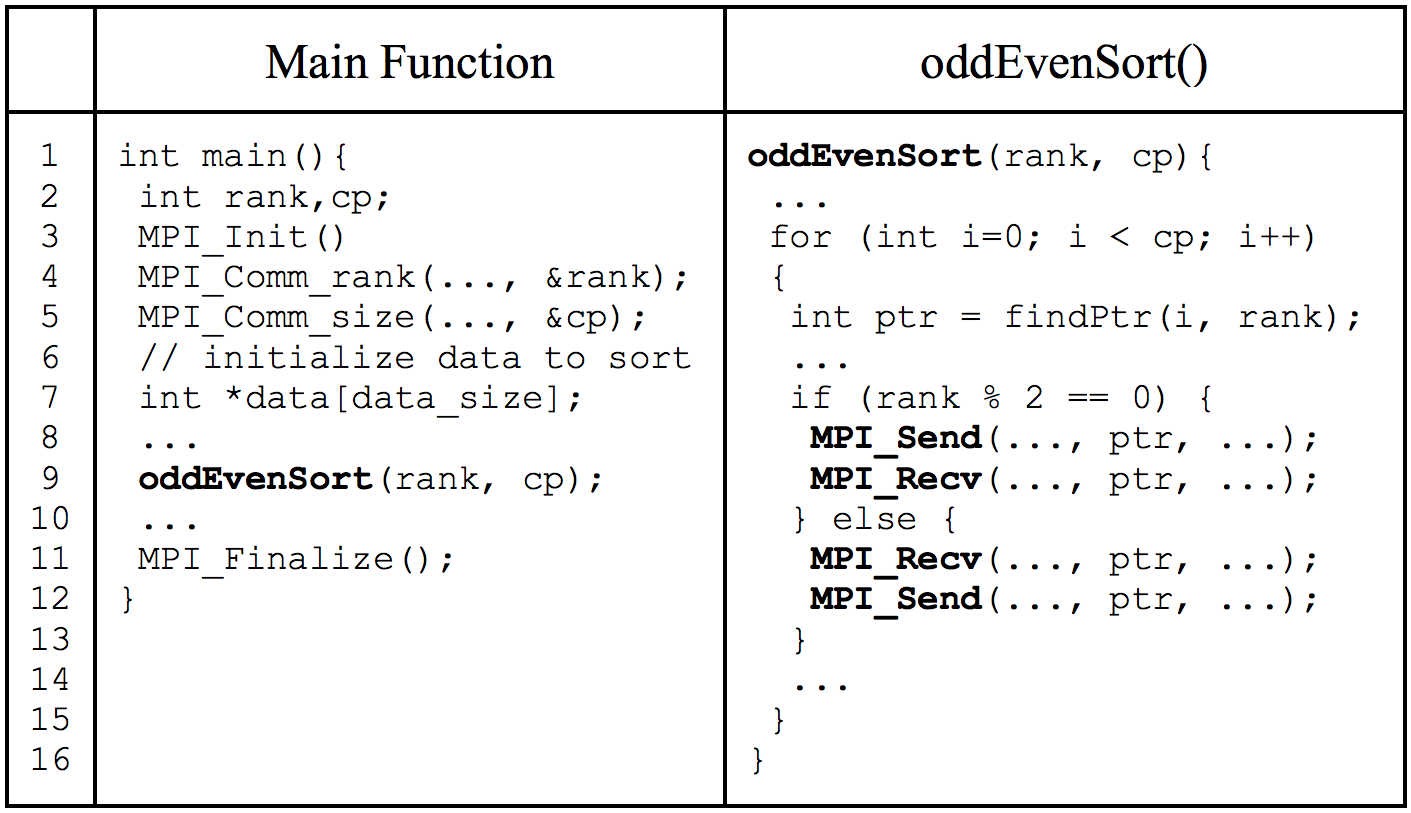
\includegraphics[width=0.40\textwidth]{figs/oddEven.png}
\label{fig.oddEven}
\end{figure}


\subsection{Example Walk-through}

We now employ
Figure~\ref{fig.oddEven}---a textbook MPI odd/even sorting example---to
illustrate DiffTrace.
%
Odd/even sorting is a parallel variant
of bubble sort
and operates in two alternating phases:
in the \textit{even phase}, the even processes exchange (conditionally swap)
values with their right neighbors, and in the \textit{odd phase},
the odd processes exchange values with their right neighbors.
%
%The for loop in line 4 of \texttt{oddEvenSort()} iterates over the phases of the algorithm. Based on the phase, the appropriate partner for each rank is computed by the function \texttt{findPtr()} (line 6). The odd/even ranks then exchange their chunks of data (lines 9-13) and sort, merge, and copy operations are performed on the received data (denoted by \texttt{...} in line 15 for simplicity).

A waiting trap in this example is this: the user may have
swapped the {\tt Recv; Send} order in the {\tt else} part,
creating head-to-head {\tt ``Send || Send''} deadlock
under low-buffering (MPI EAGER limit).
%
We will now show how DiffTrace helps picks out this root-cause.

\subsection{Pre-processing}
% Please add the following required packages to your document preamble:
% \usepackage{multirow}
\begin{table}[]
\centering
\caption{Applicable filters to PT contents based on regular expressions}
\label{tab:filters}
\scalebox{0.65}{
\begin{tabular}{|c|c|l|}
\hline
\textbf{Category} & \textbf{Sub-Category} & \multicolumn{1}{c|}{\textbf{Description}} \\ \hline
\multirow{2}{*}{Primary} & Returns & Filter out all returns \\ \cline{2-3} 
 & PLT & \begin{tabular}[c]{@{}l@{}}Filter out the ".plt" function calls for external functions/procedures that \\ their address needs to be resolved dynamically from Procedure Linkage \\ Table (PLT)\end{tabular} \\ \hline
\multirow{4}{*}{MPI} & MPI All & Only keep functions that start with "MPI\_" \\ \cline{2-3} 
 & MPI Collectives & Only keep MPI collective calls (MPI\_Barrier, MPI\_Allreduce, etc) \\ \cline{2-3} 
 & MPI Send/Recv & Only keep MPI\_Send, MPI\_Isend, MPI\_Recv, MPI\_Irecv and MPI\_Wait \\ \cline{2-3} 
 & MPI Internal Library & Keep all inner MPI library calls \\ \hline
\multirow{3}{*}{OMP} & OMP All & Only keep OMP calls (starting with GOMP\_) \\ \cline{2-3} 
 & OMP Critical & Only keep OMP\_CRITICAL\_START and OMP\_CRITICAL\_END \\ \cline{2-3} 
 & OMP Mutex & Only keep OMP\_Mutex calls \\ \hline
\multirow{4}{*}{System} & Memory & Keep any memory related functions (memcpy, memchk, alloc, malloc, etc) \\ \cline{2-3} 
 & Network & Keep any network related functions (network, tcp, sched, etc) \\ \cline{2-3} 
 & Poll & Keep any poll related functions (poll, yield, sched, etc) \\ \cline{2-3} 
 & String & Keep any string related functions (strlen, strcpy, etc) \\ \hline
\multirow{2}{*}{Advanced} & Custom & Any regular expression can be captured \\ \cline{2-3} 
 & Everything & Does not filter anything \\ \hline
\end{tabular}}
\end{table}
Using ParLoT's decoder, each trace is first decompressed.
Next, the desired functions are extracted based on predefined
(Table \ref{tab:filters}) or custom regular expressions
(i.e., \textit{filters}) and kept for later phases.
%All other trace information is discarded.
%
Table \ref{tab:oddEvenPT} shows the pre-processed traces ($T_i$) of odd/even sort with four processes.
$T_i$ is the trace that stores the function calls of process $i$.

\begin{table}[]
\centering
\caption{The generated PTs for odd/even execution with four processes}
\label{tab:oddEvenPT}
\scalebox{0.75}{
\begin{tabular}{|l|l|l|l|}
\hline
\rowcolor[HTML]{EFEFEF} 
\multicolumn{1}{|c|}{\cellcolor[HTML]{EFEFEF}\textbf{$PT_0$}} & \multicolumn{1}{c|}{\cellcolor[HTML]{EFEFEF}\textbf{$PT_1$}} & \multicolumn{1}{c|}{\cellcolor[HTML]{EFEFEF}\textbf{$PT_2$}} & \multicolumn{1}{c|}{\cellcolor[HTML]{EFEFEF}\textbf{$PT_3$}} \\ \hline \hline
... & ... & ... & ... \\ \\[-1em]  \hline
main & main & main & main \\ \\[-1em]  \hline
MPI\_Init & MPI\_Init & MPI\_Init & MPI\_Init \\ \\[-1em]  \hline
MPI\_Comm\_Rank & MPI\_Comm\_Rank & MPI\_Comm\_Rank & MPI\_Comm\_Rank \\ \\[-1em]  \hline
MPI\_Comm\_Size & MPI\_Comm\_Size & MPI\_Comm\_Size & MPI\_Comm\_Size \\ \\[-1em]  \hline
... & ... & ... & ... \\ \\[-1em]  \hline
oddEvenSort & oddEvenSort & oddEvenSort & oddEvenSort \\ \\[-1em]  \hline
... & ... & ... & ... \\ \\[-1em] \hline
findPtr & findPtr & findPtr & findPtr \\ \hline
\rowcolor[HTML]{FFCCC9} 
{\color[HTML]{333333} MPI\_Send} & \cellcolor[HTML]{CBCEFB}{\color[HTML]{333333} MPI\_Recv} & {\color[HTML]{333333} MPI\_Send} & \cellcolor[HTML]{CBCEFB}{\color[HTML]{333333} MPI\_Recv} \\ \hline
\rowcolor[HTML]{FFCCC9} 
{\color[HTML]{333333} MPI\_Recv} & \cellcolor[HTML]{CBCEFB}{\color[HTML]{333333} MPI\_Send} & {\color[HTML]{333333} MPI\_Recv} & \cellcolor[HTML]{CBCEFB}{\color[HTML]{333333} MPI\_Send} \\ \hline
... & ... & ... & ... \\ \hline
findPtr & findPtr & findPtr & findPtr \\ \hline
\rowcolor[HTML]{FFCCC9} 
{\color[HTML]{333333} MPI\_Send} & \cellcolor[HTML]{CBCEFB}{\color[HTML]{333333} MPI\_Recv} & {\color[HTML]{333333} MPI\_Send} & \cellcolor[HTML]{CBCEFB}{\color[HTML]{333333} MPI\_Recv} \\ \hline
\rowcolor[HTML]{FFCCC9} 
{\color[HTML]{333333} MPI\_Recv} & \cellcolor[HTML]{CBCEFB}{\color[HTML]{333333} MPI\_Send} & {\color[HTML]{333333} MPI\_Recv} & \cellcolor[HTML]{CBCEFB}{\color[HTML]{333333} MPI\_Send} \\ \hline
... & ... & ... & ... \\ \hline
MPI\_Finalize & MPI\_Finalize & MPI\_Finalize & MPI\_Finalize \\ \hline
\end{tabular}}
\end{table}





\begin{table}[]
\centering
\caption{NLR of Traces}
\label{tab:oddEvenPT-NLR}
\scalebox{0.75}{
\begin{tabular}{|l|l|l|l|}
\hline
\rowcolor[HTML]{EFEFEF} 
\multicolumn{1}{|c|}{\cellcolor[HTML]{EFEFEF}\textbf{$T_0$}} & \multicolumn{1}{c|}{\cellcolor[HTML]{EFEFEF}\textbf{$T_1$}} & \multicolumn{1}{c|}{\cellcolor[HTML]{EFEFEF}\textbf{$T_2$}} & \multicolumn{1}{c|}{\cellcolor[HTML]{EFEFEF}\textbf{$T_3$}} \\ \hline
MPI\_Init & MPI\_Init & MPI\_Init & MPI\_Init \\ \\[-1em]  \hline
MPI\_Comm\_Rank & MPI\_Comm\_Rank & MPI\_Comm\_Rank & MPI\_Comm\_Rank \\ \\[-1em]  \hline
MPI\_Comm\_Size & MPI\_Comm\_Size & MPI\_Comm\_Size & MPI\_Comm\_Size \\ \\[-1em]  \hline
\rowcolor[HTML]{FFCCC9} 
{\color[HTML]{333333} L0 \^{} 2} & \cellcolor[HTML]{CBCEFB}{\color[HTML]{333333} L1 \^{} 4} & {\color[HTML]{333333} L0 \^{} 4} & \cellcolor[HTML]{CBCEFB}{\color[HTML]{333333} L1 \^{} 2} \\ \hline
MPI\_Finalize & MPI\_Finalize & MPI\_Finalize & MPI\_Finalize \\ \hline
\end{tabular}}
\end{table}


\subsection{Nested Loop Representation}

Virtually all dynamic statements are found within loops.
%
Function calls within a loop body yield \textit{repetitive patterns}
in ParLoT traces.
%
Inspired by ideas for the detection of repetitive patterns in strings \cite{nakamura_fast_2013}
and other data structures \cite{kmr},
we have adapted the Nested Loop Recognition (NLR) algorithm by Ketterlin et al.~\cite{Ketterlin-nlr}
to detect repetitive patterns in ParLoT traces (cf.~Section \ref{subsec:algo-nlr}).
Detecting such patterns can be used to measure the progress of each thread,
revealing unfinished or broken loops that may be the consequence of a fault.

For example, the loop in line 3 of \texttt{oddEvenSort()} (Figure \ref{fig.oddEven}) iterates
four times when run with four processes.
Thus each $T_i$ contains four occurrences of either [\texttt{MPI\_Send}-\texttt{MPI\_Recv}] (even $i$)
or [\texttt{MPI\_Recv}-\texttt{MPI\_Send}] (odd $i$).
By keeping only MPI functions and converting each $T_i$ into its equivalent NLR,
Table \ref{tab:oddEvenPT} can be reduced to Table \ref{tab:oddEvenPT-NLR} where \textbf{L0} and \textbf{L1}
represent the \textit{loop body} [\texttt{MPI\_Send}-\texttt{MPI\_Recv}] and
[\texttt{MPI\_Recv}-\texttt{MPI\_Send}], respectively.
The integer after the \^{} symbol in NLR represents the \textit{loop iteration count}.
Note that, since the first and last processes only have one-way communication with their neighbors,
$T_0$ and $T_3$ perform only half as many iterations.

\begin{table}[]
\label{tab:sampleContext}
\caption{Context}
\scalebox{0.6}{
\begin{tabular}{l|cccccc}
 & \multicolumn{1}{l}{MPI\_Init()} & \multicolumn{1}{l}{MPI\_Comm\_Size()} & \multicolumn{1}{l}{MPI\_Comm\_Rank()} & \multicolumn{1}{l}{MPI\_Send()} & \multicolumn{1}{l}{MPI\_Recv()} & \multicolumn{1}{l}{MPI\_Finalize()} \\ \hline
Rank 0 & $\times$ & $\times$ & $\times$ &  & $\times$ & $\times$ \\
Rank 1 & $\times$ & $\times$ & $\times$ & $\times$ &  & $\times$ \\
Rank 2 & $\times$ & $\times$ & $\times$ & $\times$ &  & $\times$ \\
Rank 3 & $\times$ & $\times$ & $\times$ & $\times$ &  & $\times$
\end{tabular}}
\end{table}

\subsection{Hierarchical Clustering via FCA}
Processes in HPC applications are known to fall into predictable equivalence classes.
%
The widely used and highly successful STAT tool~\cite{stat} owes most of its
success for being able to efficiently collect stack traces (nested sequences of function
calls), organize them as prefix-trees, and equivalence the processes into teams that
evolve in different ways.
%
Coalesced stack trace graphs (CSTG, \cite{cstg}) have proven effective in
locating bugs within Uintah~\cite{uintah} and perform stat-like equivalence class formation,
albeit with the added detail of maintaining calling contexts.
%
Inspired by these ideas, FCA-based clustering provides the next logical level of refinement
in the sense that (1)~we can pick any of the multiple attributes one can mine from traces (e.g.,
pairs of function calls, memory regions accessed by processes, locks held by threads, etc.), and (2)~form this equivalencing relation quite naturally by computing the Jaccard distance between processes/threads.
%
In general,
such a classification is powerful enough to
distinguish structurally different threads from one another
(e.g., MPI processes from OpenMP threads in hybrid MPI+OpenMP applications)
and reduce the search space for bug location to a few representative classes of traces that
are distinctly dissimilar.\footnote{As emphasized earlier, we perform ``sky subtraction'' as
  in astronomy to locate comets; in our case, we diff the diffs, which is
  captured in JSM$_{D}$.}

A \textit{formal context} is a triple $K = (G, M, I)$
where $G$ is a set of \textbf{objects},
$M$ is a set of \textbf{attributes},
and $I \subseteq G \times M$ is an incidence relation that expresses
\textit{which objects have which attributes}.
Table \ref{tab:sampleContext} shows the formal context of the preprocessed odd/even-sort traces.
%
We can employ as attributes either the function calls themselves or the detected loop bodies
(each detected loop is assigned a unique ID, and one can diff with respect to these IDs).
%
The context shows that all traces include the functions MPI\_Init(),
MPI\_Comm\_size(), MPI\_Comm\_rank() and MPI\_Finalize().
The even traces contain the loop \textit{L0} and the odd traces the loop \textit{L1}.
%

% \hl{Definition of formal concept (needed?) figure }\ref{fig:formalConceptDefinition} :
% 
% \begin{figure}[]
% \centering
% \caption{Formal Concept Definition}
% 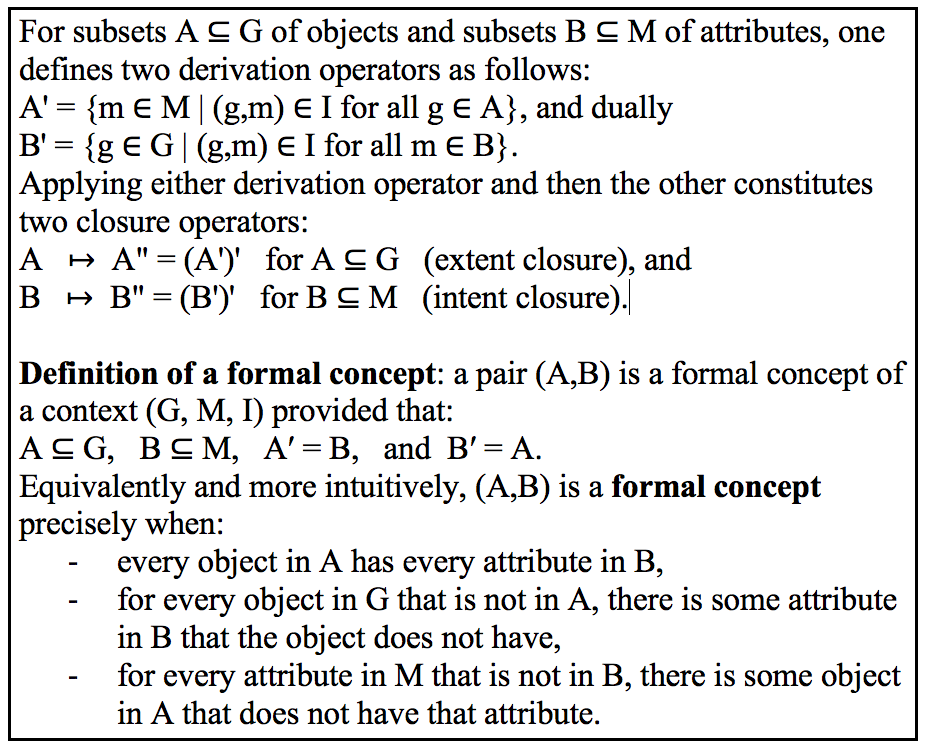
\includegraphics[width=0.45\textwidth]{figs/formalConceptDefinition.png}
% \label{fig:formalConceptDefinition}
% \end{figure}

%A \textit{concept lattice} can be derived from a \textit{formal context} by specifying \textit{formal concepts}
%(Figure \ref{fig:formalConceptDefinition})
%and a \textit{partial order} on them.
%Concept lattices are represented as a directed acyclic graph where concepts are nodes and the
%order on them determines the edges.
%
Figure \ref{fig:sampleCL} shows the concept lattice derived from the formal context in
Table~\ref{tab:sampleContext} and is interpreted as follows:

\begin{compactitem}
\item The top node indicates that all traces share MPI\_Init(),
  MPI\_Comm\_size(), MPI\_Comm\_rank() and MPI\_Finalize().
    \item The bottom node signifies that none of the traces share all attributes. 
    \item The middle nodes show that $T_0$ and $T_2$ are different from  $T_1$ and $T_3$.
\end{compactitem}



% Once the redundant labels are removed from the lattice, each object (trace) and attribute appears in the lattice exactly once. Consequently, the nodes of the lattice form the desired grouping, since it is guaranteed that each trace belongs to exactly one group. However, the concept lattice itself does not provide similarity values for the distinct groups of traces. The \textit{Jaccard Index}, also known as \textit{Intersection over Union}, measures the \textit{distance} between sets $A$ and $B$ in terms of the ratio of the \textit{intersection} size of $A$ and $B$ over the size of their \textit{union}.
% 

%


\begin{figure}[t]
\centering
\scalebox{0.5}{
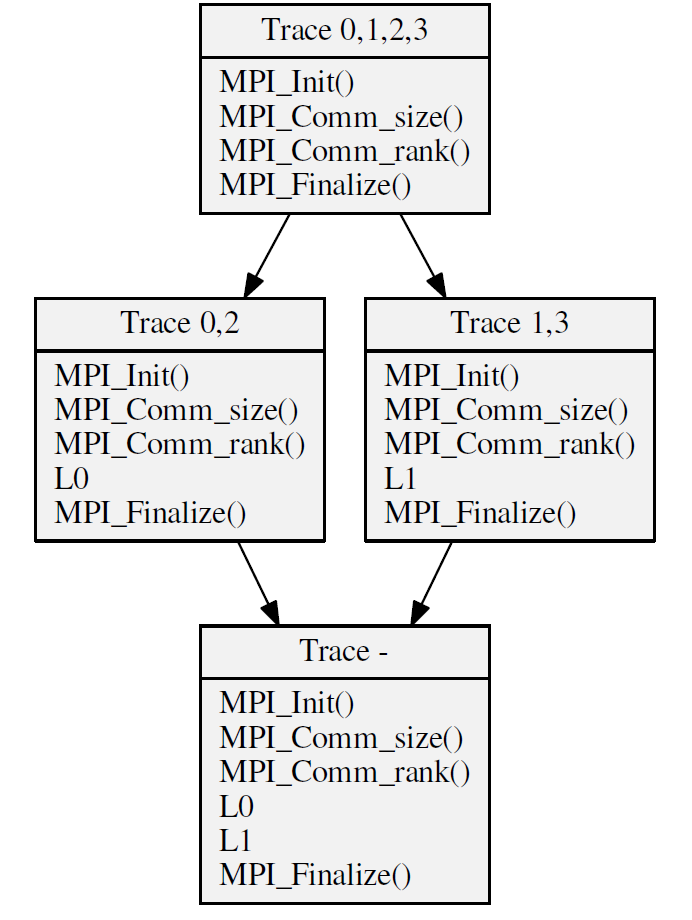
\includegraphics[width=3.4in]{figs/sampleCL.png}}
\caption{Sample Concept Lattice from Object-Attribute Context in Table \ref{tab:sampleContext}}
\label{fig:sampleCL}
\end{figure}


%\begin{figure}[]
%\centering
%\scalebox{0.8}{
%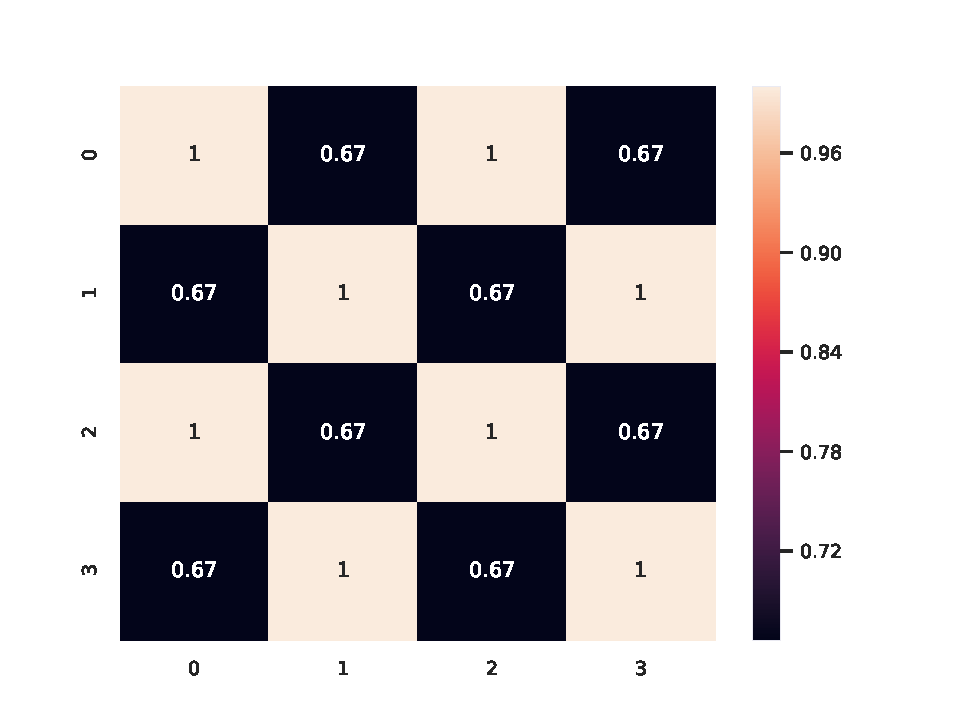
\includegraphics[width=3.4in]{figs/oddEvenJSM.pdf}}
%\caption{Pairwise Jaccard Similarity Matrix (JSM) of MPI processes in sample code}
%\label{fig:jsm}
%\end{figure}

\begin{figure}[]
\centering
\scalebox{0.8}{
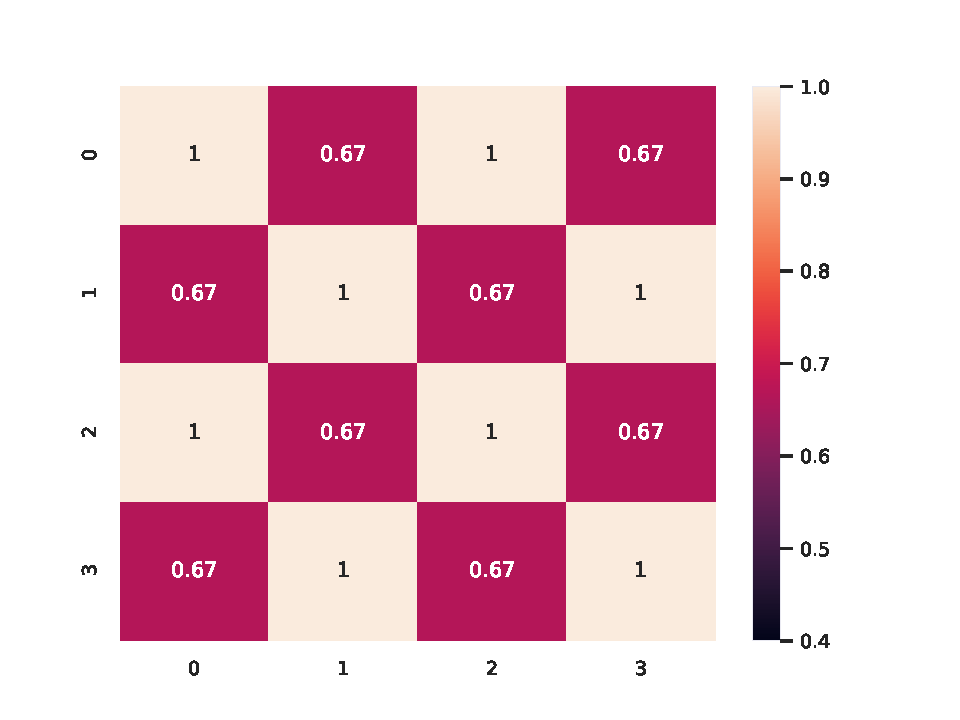
\includegraphics[width=3.4in]{figs/oddEvenJSM2.pdf}}
\caption{Pairwise Jaccard Similarity Matrix (JSM) of MPI Processes in Sample Code}
\label{fig:jsm2}
\end{figure}

% For any pair of $(T_i, T_j)$, the number of attributes in the Lowest Common Ancestor (LCA) node of $T_i$ and $T_j$ in the lattice is the number of attributes that $T_i$ and $T_j$ have in common (intersection). The sum of the number of attributes of the nodes on the path from each $T_i$ and $T_j$ to their LCA is the union. This property is one of the motivations for using concept lattices as classifier since it makes computing the union and intersection easy and fast.
% 
% Some algorithms for extracting concepts from contexts and constructing the concept lattice require the whole context to be present in the memory.
%

The complete pairwise Jaccard Similarity Matrix (JSM) can easily be computed from concept lattices.
%
For large-scale executions with thousands of threads, it is imperative
to employ incremental algorithms to
construct concept lattices (detailed in Section \ref{subsec:algo-cl}).
%
% Through an incremental concept-lattice-construction approach,
% DiffTrace extracts attributes (\hl{table that shows attributes})
% from NLR traces and injects them into a concept lattice one trace at a time 
%
Figure \ref{fig:jsm2}
shows the heatmap
% (explain this)
of the JSM obtained from the concept lattice in Figure \ref{fig:sampleCL}.
%
DiffTrace uses the JSM to form equivalence classes of traces by hierarchical clustering.
%
Next, we show how the differences between two hierarchical clusterings from two executions
(faulty vs.~normal) reveal which traces have been affected the most by the fault.


\subsection{Detecting Suspicious Traces via JSM$_{D}$}
% So far,
% we have explained how DiffTrace can narrow down the search space from numerous long traces to just a few equivalent JSMs (i.e., clusters).
% %
JSM$_{normal}$[i][j] (JSM$_{faulty}$[i][j]) shows the Jaccard similarity score of $T_i$ and $T_j$ from the normal trace ($T_i^\prime$ and $T_j^\prime$).
% 
% However, we are interested in detecting what changed the most due to the fault.
% with respect to the ``natural asymmetry'' of the application.
%
%In other words, DiffTrace abstracts function call traces into JSMs, which are reflections of asymmetry among traces.
As explained earlier, we compute
JSM$_{D}$ to detect outlier executions, where
JSM$_{D}$ = $|$JSM$_{faulty} - $JSM$_{normal}|$.

%
We sort the suggestion table based on the \textit{B-score}
similarity metric of two hierarchical clusterings \cite{fowlkes83} (cf.~Section \ref{subsec:algo-bscore}).
%
A single iteration through the
DiffTrace loop
(with a single set of parameters shown as a dashed box in Figure \ref{fig.diffTraceOverview})
may still not detect the root-cause of a bug.
%
The user can then (1)~alter the linkage method employed in computing the hierarchical clustering
(reorder the dendrograms built to achieve the clustering),
(2)~alter the FCA attributes, (3)~adjust the NLR constants (loops are extracted with
realistic complexity by observing repetitive patterns inside a preallocated buffer),
and/or (4)~the front-end filters.
%
This is shown in the iterative loop in
Figure \ref{fig.diffTraceOverview}.

\subsection{Evaluation}

%The resulting outlier traces are candidates for the potential cause of the change in the program behavior and thus, a potential fault root cause or fault manifestation.
%

%
%Also, a different set of parameters might produce inaccurate suggestions (false positives).
%

\begin{figure}

     \centering
     \begin{subfigure}[b]{0.15\textwidth}
        \centering
		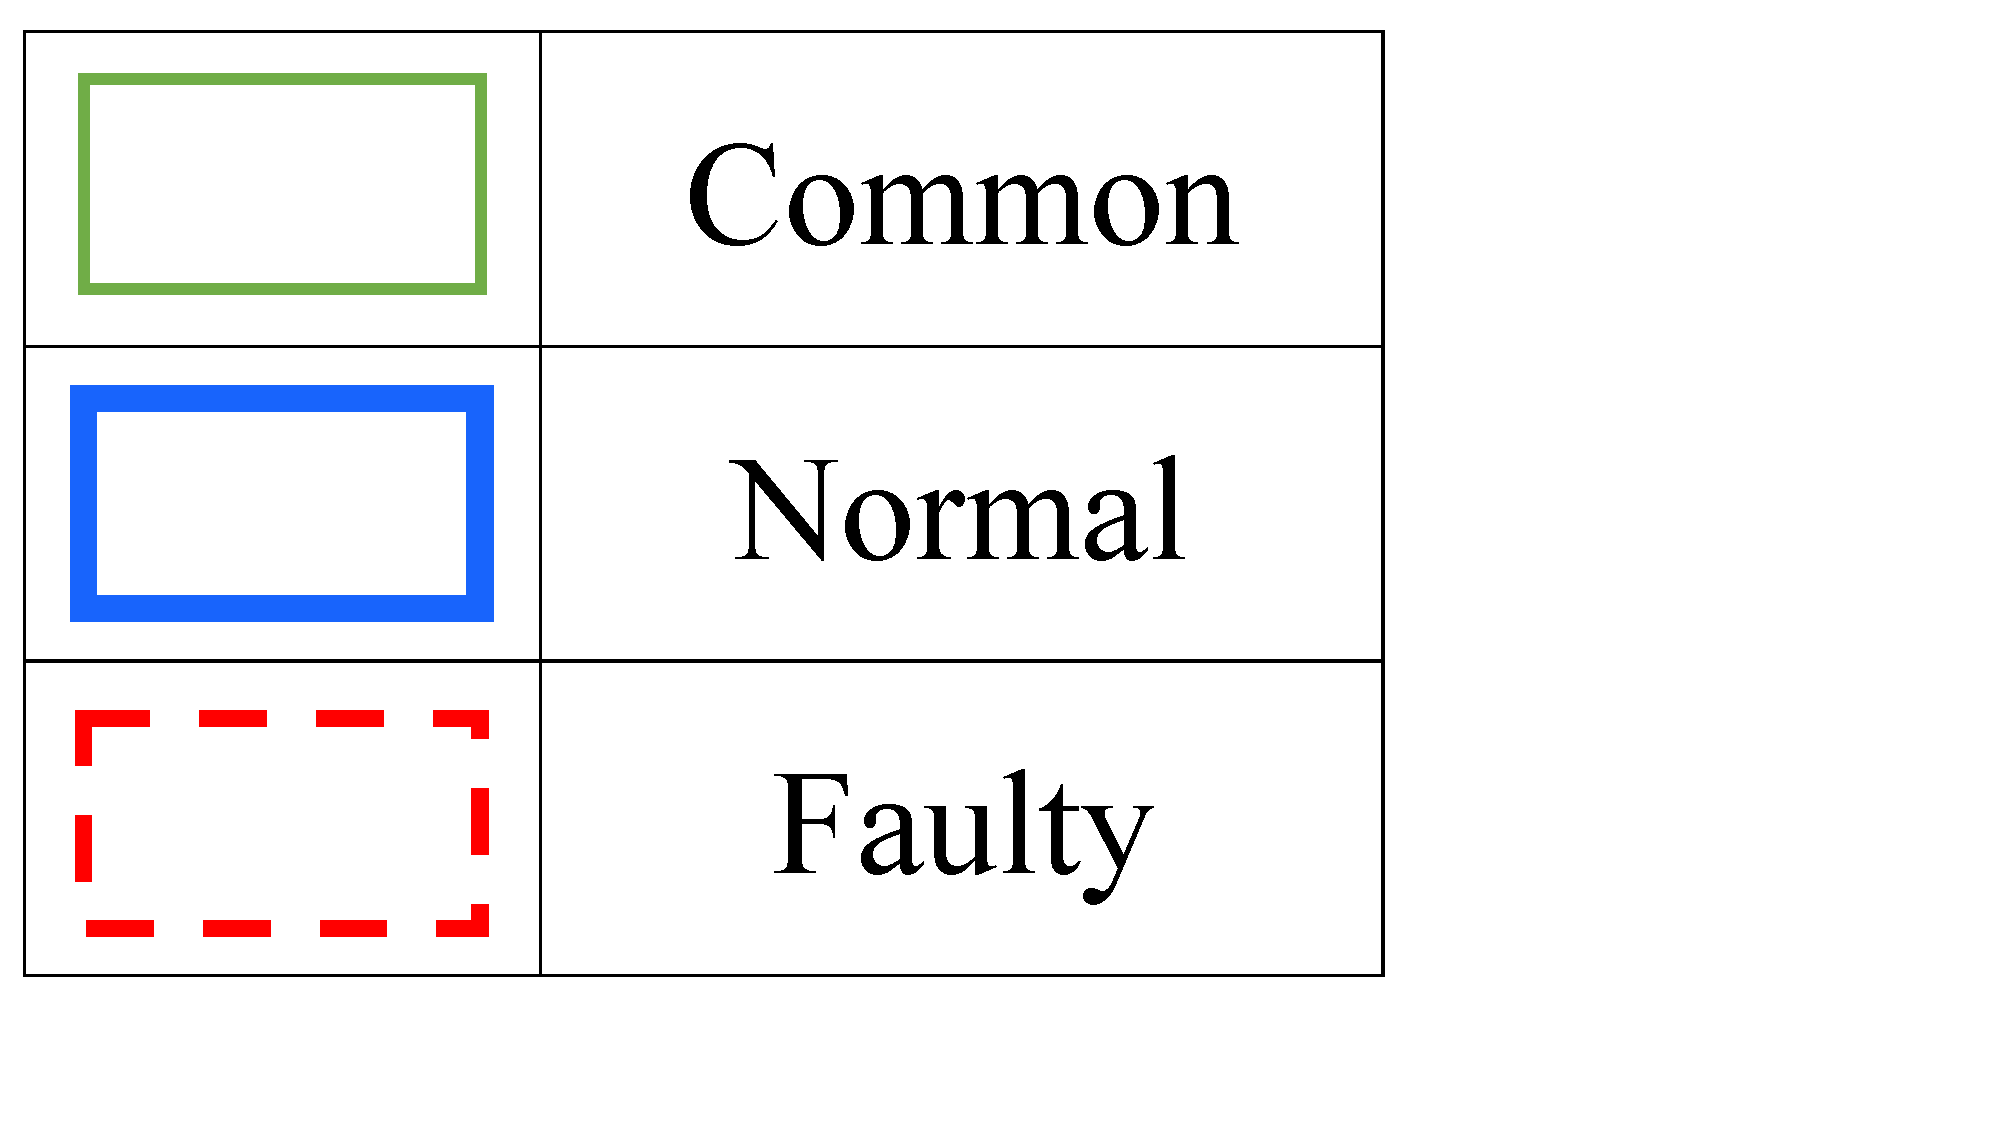
\includegraphics[width=\textwidth]{figs/legend.pdf}
		\caption{Legend}
		\label{fig:legend}
	\end{subfigure}
	     \hfill
     \begin{subfigure}[b]{0.31\textwidth}
         \centering
\includegraphics[width=\textwidth]{figs/{b-11.mpi.0K10-5}.pdf}
\caption{swapBug}
\label{fig:swapbug}
     \end{subfigure}
\caption{diffNLR Example}
\label{fig:sampleDiffNLR}

\end{figure}

To evaluate the effectiveness of DiffJSM, we planted two artificial bugs (\textit{swapBug}
and \textit{dlBug}) in the code from Figure \ref{fig.oddEven} and ran it with 16 processes.
%
\textit{swapBug} swaps the order of MPI\_Send and MPI\_Recv in rank 5
after the seventh iteration of the loop in line 3 of \texttt{oddEvenSort},
simulating a potential deadlock. \textit{dlBug} simulates an actual deadlock in the same location
(rank 5 after the seventh iteration).
%
Upon collection of ParLoT traces from the execution of the buggy code versions,
DiffTrace first decompresses them and filters out all non-MPI functions.
Then two major loops are detected, \textbf{L0} and \textbf{L1} (identical to the ones in Table \ref{tab:oddEvenPT-NLR}),
that are supposed to loop 16 times in the even and odd traces,
respectively (except for the first and last traces, which loop just eight times).

After constructing concept lattices and their corresponding JSMs, trace 5 appears as the trace that got
affected the most by the bugs because row 5 (showing the similarity score of $T_5$ relative to all other traces)
(JSM$_{normal}$[5][i] for $i \in [0,16)$)
  changed the most after the bug was introduced.
  %Consequently, it means that $T^\prime_5$ affected the asymmetry of all $T_i$s.
%
The differences between the suggested suspicious trace ($T^\prime_s$)
and its corresponding normal trace ($T_s$) is visualized by \textit{diffNLR}.


\subsubsection{diffNLR}
To highlight the differences in an easy-to-understand manner, DiffTrace visually separates the common and different blocks of a pair of pre-processed traces via \textit{diffNLR}, a graphical visualization of the \texttt{diff} algorithm \cite{diff-myers}.
%





\begin{figure}[t]
\centering
\includegraphics[width=0.3\textwidth]{figs/{adl-11.mpi.0K10-5}.pdf}
\caption{dlBug}
\label{fig:dlbug}
\end{figure}
\texttt{diff} takes two sequences $S_A$ and $S_B$ and computes the minimal \textit{edit} to convert $S_A$ to $S_B$. This algorithm is used in the GNU \texttt{diff} utility to compare two text files and in git for efficiently keeping track of file changes.
Since ParLoT preserves the order of function calls, each trace $T_i$ is totally ordered. Thus \textit{diff} can expose the differences of a pair of $T$s. \textit{diffNLR} aligns common and different blocks of a pair of sequences (e.g., traces) horizontally and vertically, making it easier for the analyst to see the differences at a glance.
For simplicity, our implementation of \textit{gdiff} only takes one argument $x$ that denotes \textit{the suspicious trace}.

diffNLR$(x) \equiv $ diffNLR$(T_x,T_x^\prime)$
%
where $T_x$ is the trace of thread/process $x$ of a normal execution and $T^\prime_x$ is the corresponding trace of the faulty execution.

Figure \ref{fig:swapbug} shows the diffNLR(5) of \textit{swapBug} where $T_5$ iterates over the loop [MPI\_Recv - MPI\_Send] 16 times (L1\^{}16) after the MPI initialization while the order swap is well reflected in $T_5^\prime$ (L1\^{}7 - L0\^{}9). Both processes seem to terminate fine by executing MPI\_Finalize(). 
However, diffNLR(5) of \textit{dlBug} (Figure \ref{fig:dlbug}) shows that, while $T_5$ executed MPI\_Finalize, $T_5^\prime$ got stuck after executing L1 seven times and never reached MPI\_Finalize.

This example illustrates how our approach can locate the part of each execution that was impacted by a fault. Having an understanding of \textit{how the application should behave normally} can reduce the number of iterations by picking the right set of parameters sooner. 


%\begin{figure}[]
%\centering
%\caption{A line change in oddEvenSort (left) that might cause a deadlock in oddEvenSort\_DL (right)}
%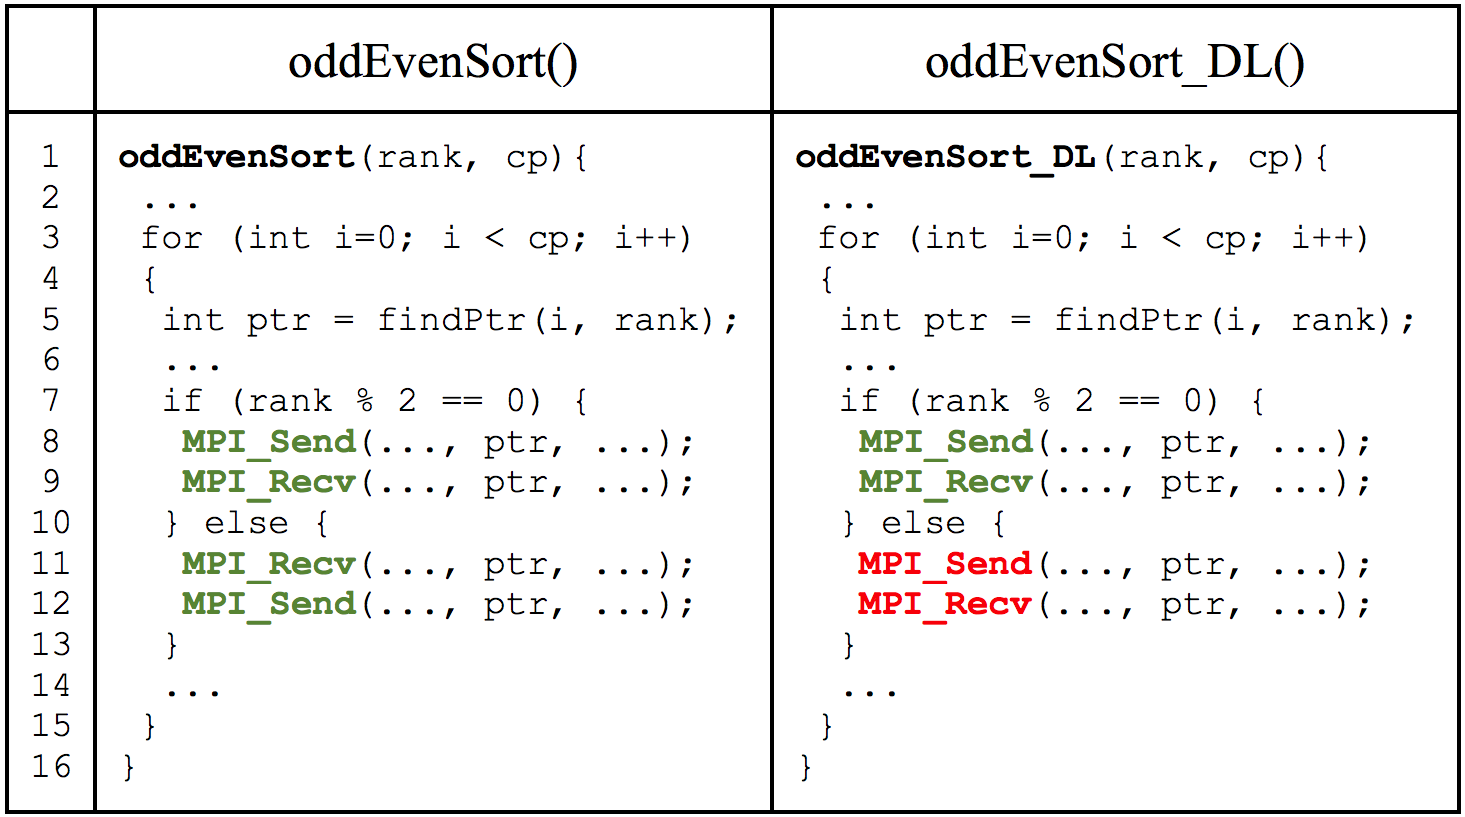
\includegraphics[width=0.45\textwidth]{figs/oddEvenDL.png}
%\label{fig.oddEvenDL}
%\end{figure}







